\iffalse
\chapter{2018}
\section{ph}
\author{EE24BTECH11030}
\fi
\item The elementary particle $\Xi^0$ is placed in the baryon decuplet, shown below, at
\begin{figure}[!ht]
    \centering
    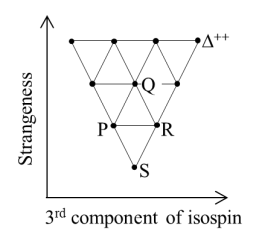
\includegraphics[scale=0.4]{GATE-yearwise/GATE(8)/figs/fig1.png}
    \caption{}
    \label{fig:50,51}
\end{figure}
\begin{multicols}{2}
\begin{enumerate}
    \item P
    \item Q
    \item R
    \item S
\end{enumerate}
\end{multicols}

\bigskip

\item The intrinsic/permanent electric dipole moment in the ground state of hydrogen atom is $(a_0$ is the Bohr radius$)$
\begin{multicols}{2}
\begin{enumerate}
    \item $-3 e a_0$
    \item zero
    \item $e a_0$
    \item $3 e a_0$
\end{enumerate}
\end{multicols}

\bigskip

\item The high temperature magnetic susceptibility of solids having ions with magnetic moments can be described by $\chi \propto \frac{1}{T + \theta}$ with $T$ as absolute temperature and $\theta$ as constant. The three behaviors i.e. paramagnetic, ferromagnetic and anti-ferromagnetic are described, respectively, by
\begin{multicols}{2}
\begin{enumerate}
    \item $\theta < 0$, $\theta > 0$, $\theta = 0$
    \item $\theta > 0$, $\theta < 0$, $\theta = 0$
    \item $\theta = 0$, $\theta < 0$, $\theta > 0$
    \item $\theta = 0$, $\theta > 0$, $\theta < 0$
\end{enumerate}
\end{multicols}

\bigskip

\item Which one of the following is an allowed electric dipole transition?
\begin{multicols}{2}
\begin{enumerate}
    \item ${}^1 S_0 \rightarrow {}^3 S_1$
    \item ${}^2 P_{3/2} \rightarrow {}^2 D_{5/2}$
    \item ${}^2 D_{5/2} \rightarrow {}^2 P_{1/2}$
    \item ${}^3 P_0 \rightarrow {}^5 D_0$
\end{enumerate}
\end{multicols}

\bigskip

\item In the decay, $\mu^+ \rightarrow e^+ + \nu_e + X$, what is $X$?
\begin{multicols}{2}
\begin{enumerate}
    \item $\gamma$
    \item $\bar{\nu_e}$
    \item $\nu_\mu$
    \item $\bar{\nu_\mu}$
\end{enumerate}
\end{multicols}

\bigskip

\item A spaceship is traveling with a velocity of $0.7 c$ away from a space station. The spaceship ejects a probe with a velocity $0.59 c$ opposite to its own velocity. A person in the space station would see the probe moving at a speed $X c$, where the value of $X$ is \underline{\hspace{2cm}} (up to three decimal places).

\bigskip

\item For an operational amplifier (ideal) circuit shown below,\\
\begin{figure}[!ht]
\centering
\resizebox{1\textwidth}{!}{%
\begin{circuitikz}
\tikzstyle{every node}=[font=\normalsize]
\draw (12,17.75) to[short] (12,17.25);
\draw (12,17.75) to[short] (13.25,17.75);
\draw (12,16.75) to[short] (13.25,16.75);
\draw (13.25,18.25) to[short] (13.25,16.25);
\draw (13.25,18.25) to[short] (14.25,17.25);
\draw (13.25,16.25) to[short] (14.25,17.25);
\draw (13.75,17.75) to[short] (13.75,18.25);
\draw (13.75,16.75) to[short] (13.75,16.25);
\draw (14.25,17.25) to[short] (16.5,17.25);
\draw (15.25,18.75) to[short] (15.25,17.25);
\draw (12.25,18.75) to[short] (12.25,17.75);
\draw (16,17.25) to[R=$R_{L}$] (16,15.75);
\draw (12.25,18.75) to[R=4k$\Omega$] (15.25,18.75);
\draw (10,17.75) to[R=2k$\Omega$] (12,17.75);
\draw (10,17.25) to[R, l_=5k$\Omega$] (12,17.25); % Moved label below the resistor
\draw (16,15.75) to (16.25,15.75) node[ground]{};
\draw (12,16.75) to (12.25,16.75) node[ground]{};
\node [font=\normalsize] at (17,17.25) {$V_{0}$};
\node [font=\normalsize] at (9.75,17.75) {$V_{1}$};
\node [font=\normalsize] at (9.75,17.25) {$V_{2}$};
\node [font=\small] at (13.75,16) {-10V};
\node [font=\small] at (14.25,18.25) {+10V};
\node [font=\normalsize] at (13.5,17.75) {-};
\node [font=\normalsize] at (13.5,16.75) {+};
\end{circuitikz}
}%
\end{figure}

     if $V_1 = 1 \, \text{V}$ and $V_2 = 2 \, \text{V}$, the value of $V_0$ is \underline{\hspace{2cm}} V (up to one decimal place).
        
    \bigskip

\item An infinitely long straight wire is carrying a steady current $I$. The ratio of magnetic energy density at distance $r_1$ to that at $r_2 (= 2 \, r_1)$ from the wire is \underline{\hspace{2cm}}.
    \bigskip

\item A light beam of intensity $I_0$ is falling normally on a surface. The surface absorbs 20\% of the intensity and the rest is reflected. The radiation pressure on the surface is given by $X \frac{I_0}{c}$, where $X$ is \underline{\hspace{2cm}} (up to one decimal place). Here $c$ is the speed of light.
    \bigskip

\item The number of independent components of a general electromagnetic field tensor is \underline{\hspace{2cm}}.
    \bigskip

\item If $X$ is the dimensionality of a free electron gas, the energy $(E)$ dependence of density of states is given by $E^{\frac{X}{2}-Y}$, where $Y$ is \underline{\hspace{2cm}}.
    \bigskip

\item For nucleus $^{164}\text{Er}$, a $J^{\pi} = 2^+$ state is at 90 keV. Assuming $^{164}\text{Er}$ to be a rigid rotor, the energy of its $4^+$ state is \underline{\hspace{2cm}} keV (up to one decimal place).

\bigskip

\item Given $\vec{V}_1 = \hat{i} - \hat{j}$ and $\vec{V}_2 = -2\hat{i} + 3\hat{j} + 2\hat{k}$, which one of the following $\vec{V}_3$ makes $(\vec{V}_1, \vec{V}_2, \vec{V}_3)$ a complete set for a three dimensional real linear vector space?
\begin{enumerate}
    \begin{multicols}{2}
        \item[(A)] $\vec{V}_3 = \hat{i} + \hat{j} + 4\hat{k}$
        \item[(B)] $\vec{V}_3 = 2\hat{i} - \hat{j} + 2\hat{k}$
        \item[(C)] $\vec{V}_3 = \hat{i} + 2\hat{j} + 6\hat{k}$
        \item[(D)] $\vec{V}_3 = 2\hat{i} + \hat{j} + 4\hat{k}$
    \end{multicols}
\end{enumerate}

